\section{Simulačný model}
Simulačný model bol vytvorený v prostredí Simulink s využitím predlohy z knižnice Simulinku \textit{Synchronous Machine}, ktorá bola využívaná počas cvičení. Bloková schéma simulačného modelu je zobrazená na obrázku \ref{fig:simulacny_model}. Model pozostáva z modelu synchrónneho generátora (blok Synchronous Machine), modelu vodnej turbíny (blok HTG),modelu budiča ST4C, ktorým bol nahradený pôvodný model budiča (Excitation
System), trojfázového transformátora (blok Three-Phase Transformer) a záťaže. Blok trojfázového skratovača (Three-Phase Fault) bol pre účely tohto zadania vypnutý.


\begin{figure}[h]
    \centering
    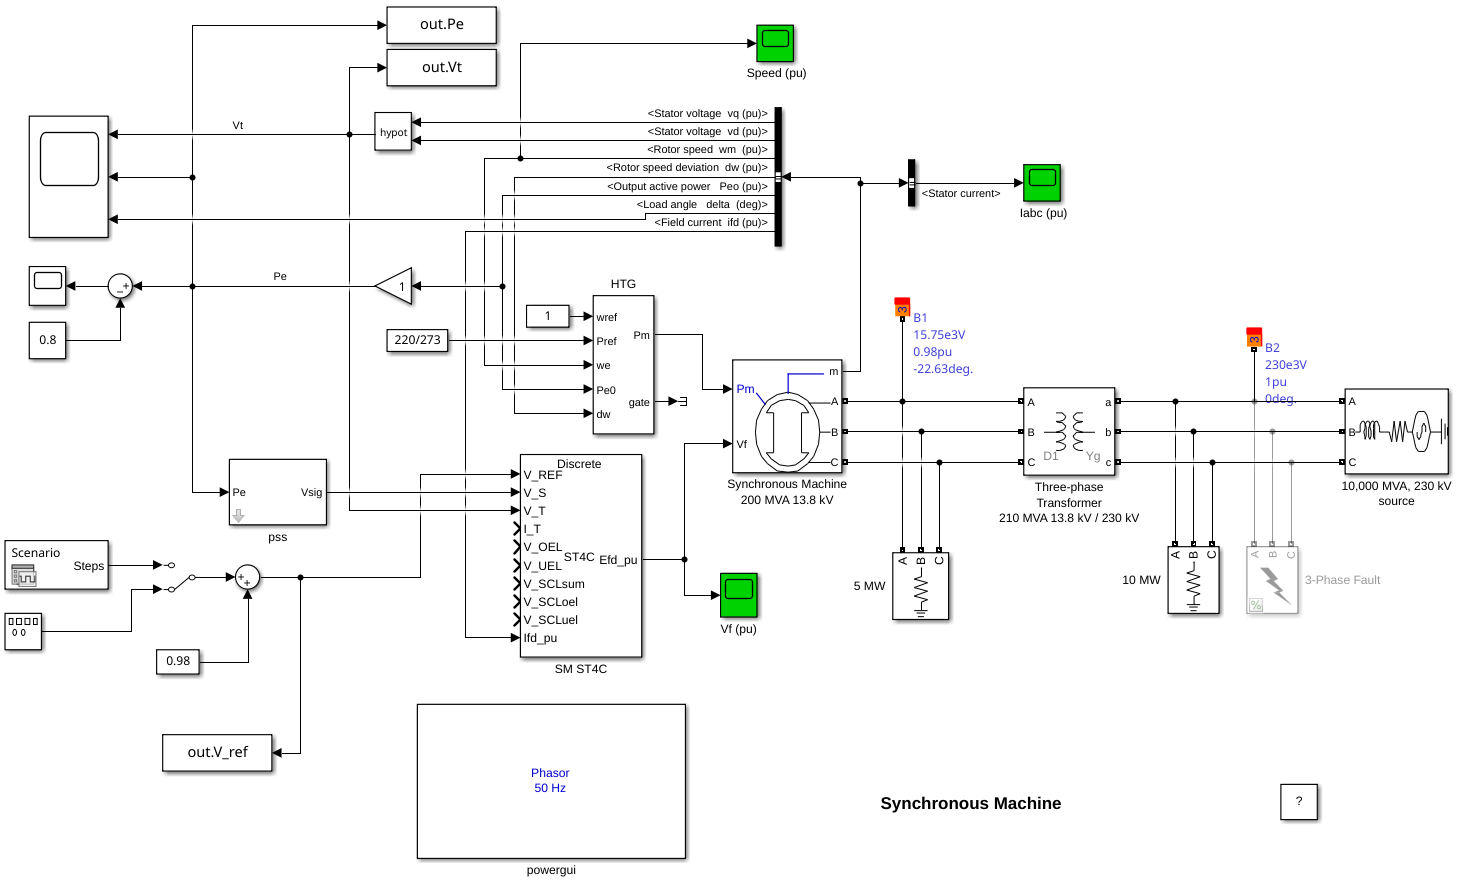
\includegraphics[width=1\textwidth]{img/Simulink_model.png}
    \caption{Bloková schéma simulačného modelu v Simulinku}
    \label{fig:simulacny_model}
\end{figure}

\subsection{Model synchrónneho generátora}
Synchrónny generátor je modelovaný pomocou bloku Synchronous Machine s nominálnym zdanlivým výkonom $S_n = 273 MVA$, činným výkonom $P = 220 MW$ a nominálnym napätím $U_n = 15.75 kV$. Všetky parametre modelu synchrónneho generátora sú uvedené v tabuľke \ref{tab:parametre_sg}. Na základe týchto parametrov boli upravené aj parametre ostaných blokov, ako napríklad transformátor a Load Flow Bus, aby zodpovedali požiadavkám zadania.

\begin{table}[htbp]
    \centering
    \begin{tabular}{llc}
        \hline
        Názov & Jednotka & SG1 \\
        \hline
        Sn & [MVA] & 273 \\
        Typ stroja & - & Hladký rotor \\
        $U_n$ & [kV] & 15.75 \\
        P & [MW] & 220 \\
        $R_{st}$ & [p.u.] & 0.0016 \\
        $x_d''$ & [p.u.] & 0.185 \\
        $x_d$ & [p.u.] & 1.7 \\
        $x_q$ & [p.u.] & 1.62 \\
        $x_d'$ & [p.u.] & 0.245 \\
        $x_q'$ & [p.u.] & 0.256 \\
        $x_q''$ & [p.u.] & 0.155 \\
        $x_l$ & [p.u.] & 0.147 \\
        $T_{do}'$ & [s] & 4.8 \\
        $T_{do}''$ & [s] & 0.023 \\
        $T_{qo}'$ & [s] & 0.5 \\
        $T_{qo}''$ & [s] & 0.02 \\
        H & [s] & 4.56 \\
        \hline
    \end{tabular}
    \caption{Parametre SG}
    \label{tab:parametre_sg}
\end{table}
 

\subsection{Model vodnej turbíny}
Model vodnej turbíny je realizovaný pomocou bloku HTG (Hydraulic Turbine and Governor), v ktorom sú nastavené východzie parametre. Neskôr boli parametre regulátora turbíny $K_p$ a $K_i$ upravené v rámci optimalizácie parametrov regulátorov, ktorá je popísaná v kapitole \ref{sec:optimalizacia}.

\subsection{Stabilizátor PSS}
Stabilizátor PSS (Power System Stabilizer) bol pridaný do modelu s cieľom zlepšiť stabilitu systému. Porovnanie prebehov simulácie bez použitia PSS a s použitím PSS je zobrazené na obrázku \ref{fig:pss_comparison}. 


\begin{figure}[h]
    \centering
    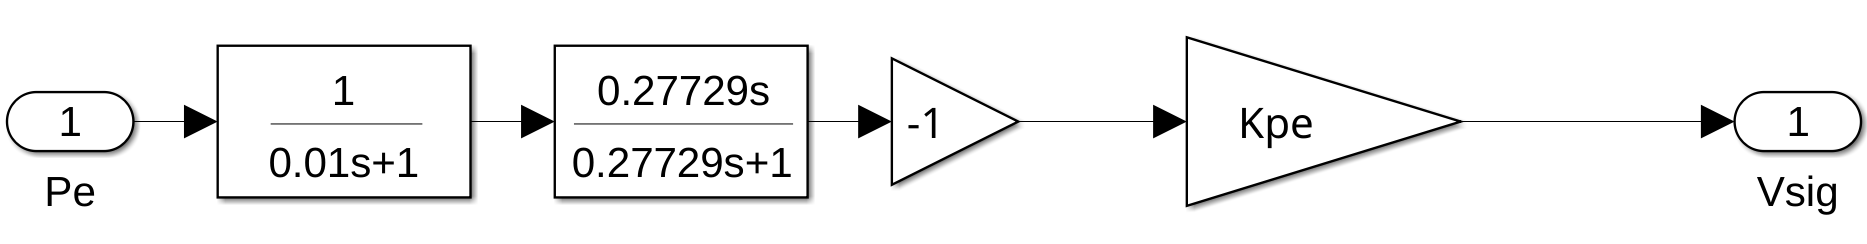
\includegraphics[width=0.8\textwidth]{img/PSS_model.png}
    \caption{Bloková schéma stabilizátora PSS v Simulinku}
    \label{fig:pss_model}
\end{figure}


\begin{figure}[htbp]
    \centering
    \begin{subfigure}[b]{0.48\textwidth}
        \centering
        \includegraphics[width=\textwidth]{example-image-a} % zmeňte na img/vas_obrazok_bez_pss.png
        \caption{Priebeh bez použitia PSS}
        \label{fig:pss_bez}
    \end{subfigure}
    \hfill
    \begin{subfigure}[b]{0.48\textwidth}
        \centering
        \includegraphics[width=\textwidth]{example-image-b} % zmeňte na img/vas_obrazok_s_pss.png
        \caption{Priebeh s použitím PSS}
        \label{fig:pss_s}
    \end{subfigure}
    \caption{Porovnanie prebehov simulácie bez a s použitím PSS}
    \label{fig:pss_comparison}
\end{figure}

Ako je možné vidieť z obrázku \ref{fig:pss_comparison}, použitie stabilizátora PSS výrazne zlepšilo stabilitu systému, čo sa prejavilo v rýchlejšom tlmení oscilácií a menšom kmitaní napätia a činného výkonu. Týmto sa potvrdila účinnosť stabilizátora PSS v zlepšení dynamického správania systému a zvýšení jeho odolnosti voči poruchám. 